\documentclass[12pt,addpoints]{guia}
\grado{2$^\circ$ de Secundaria}
\cicloescolar{2022-2023}
\materia{Ciencias y Tecnología: Física}
\guia{10}
\unidad{3}
\title{Grupos de galaxias}
\aprendizajes{\item Describe cómo se lleva a cabo la exploración de los cuerpos celestes por medio de la detección
de las ondas electromagnéticas que emiten.\item Describe algunos avances en las características
y composición del Universo (estrellas, galaxias y otros sistemas).}
\author{JC Melchor Pinto}
\begin{document}
\INFO%
\begin{sectionbox}{Grupos de galaxias}
    \begin{wrapfigure}[23]{l}[1mm]{0.45\textwidth}
        \centering
        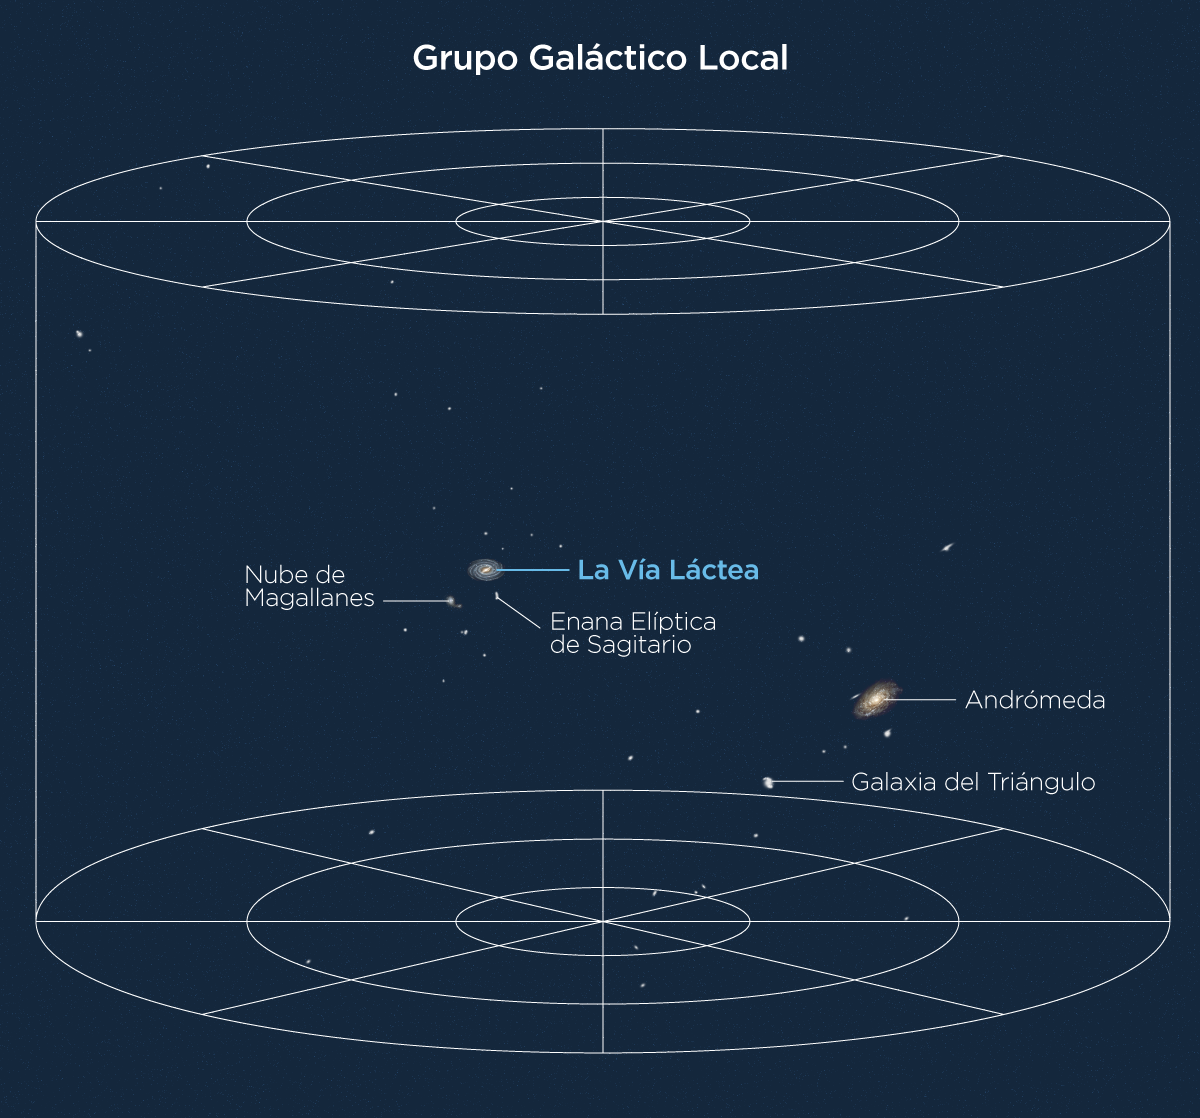
\includegraphics[width=\linewidth]{../images/grupogalacticolocal}
        \caption{Esquema del Grupo Local de galaxias.}
        \label{fig:grupogalacticolocal}
    \end{wrapfigure}
    A escalas mayores, las galaxias tienden a formar grupos
    que sólo hasta años recientes ha sido posible observar
    y analizar.
    La Vía Láctea, y unas 30 galaxias forman el llamado
    \textbf{Grupo Local}. Nuestra galaxia tiene algunas galaxias satélites, entre ellas las dos Nubes de Magallanes, que se
    pueden observar a simple vista desde el hemisferio sur
    de la Tierra; también Sagitario, una galaxia elíptica enana descubierta hasta 1994 debido a que se encuentra en
    la dirección del plano galáctico, donde el polvo absorbe la
    luz y dificulta la observación astronómica. La galaxia
    satélite más cercana a la Vía Láctea es la enana del Can
    Mayor, ubicada a unos 25,000 años luz de la Tierra. Se
    considera que nuestra galaxia está en proceso de engullir gravitacionalmente a sus galaxias satélites. La galaxia
    más grande del Grupo Local es M31, conocida como la
    Gran Nebulosa de Andrómeda (figura \ref{fig:grupogalacticolocal}).
   
    La Vía Láctea y unas 14 galaxias
    gigantes integran una estructura en
    forma de anillo conocida como
    \textbf{Concilio de Gigantes} (figura \ref{fig:20230520234809}). El
    Grupo Local está cerca del centro y
    el conjunto se mueve en torno a él.
    Los ejes de rotación de las galaxias
    que integran el Concilio de Gigantes
    coinciden, por lo cual se cree que tienen un origen común. En esta escala
    el año luz empieza a quedarse pequeño, y resulta más práctico utilizar otra
    unidad de longitud.



    Las galaxias integran pequeños grupos, como los antes
    descritos para la Vía Láctea, y también forman \textbf{cúmulos
    de galaxias}. Los cúmulos tienen tamaños típicos de 2 a
    3 Mpc y la rapidez de las galaxias que los conforman
    están en un rango de 400 a 1,400 km/s. Los cúmulos fueron reconocidos y catalogados por primera vez por
    \textbf{George Abell (1927-1983)} en el observatorio de Monte
    Palomar, California, Estados Unidos de América.
    Entre los cúmulos más cercanos a la Vía Láctea está el
    de Virgo, a unos 20 Mpc, compuesto por unas 1,300 galaxias,
    y el de Coma, situado cerca del polo norte galáctico, a unos 100 Mpc, conformado por unas 1 000 galaxias.

    

    Los cúmulos no son meras agrupaciones de galaxias, sino que forman una entidad fisica. Esto se ha comprobado al estudiar el gas intergalactico en el interior de los cumulos y la manera en que las galaxias se distribuyen en ellos. Las galaxias espirales abundan más en la periferia y las elípticas y lenticulares proliferan en las regiones centrales, lo cual indica que las galaxias centrales interactuan más con el polvo intergalactico del cúmulo. En el centro del \label{087b_a}cúmulo también son frecuentes las fusiones de galaxias, lo cual lleva en ocasiones a formar galaxias elípticas gigantes, conocidas como \textbf{galaxias cD} o \textbf{galaxias centrales dominantes} (como la galaxia IC 1101 que ya se mencionó).
    \begin{wrapfigure}[18]{r}[1mm]{0.5\textwidth}
        \centering
        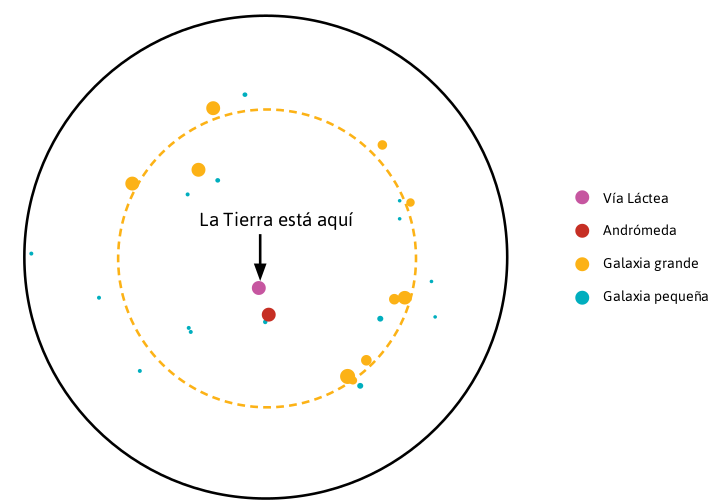
\includegraphics[width=\linewidth]{../images/20230520234809}
        \caption{Esquema del Concilio de Gigantes.}
        \label{fig:20230520234809}
    \end{wrapfigure}

    Los cúmulos de galaxias, a su vez, integran \label{087b_b}\textbf{supercúmulos} y en este punto comienza la denominada gran escala del Universo, que pudiste apreciar en la figura \ref{fig:grupogalacticolocal}. Los supercumulos se agrupan alineandose en \label{087b_c}\textbf{filamentos}, a veces en grandes \textbf{paredes}. Los filamentos se unen en vertices formando una red que muestra enormes \label{087b_d}vacios conocidos como \textbf{vacios cósmicos}.
    Hasta ahora ha sido posible identificar una estructura a la cual
    pertenece el supercúmulo local del que forma parte nuestra galaxia y se conoce como Laniakea (\comillas{cielo inmenso}, en hawaiano).
    Para terminar esta panorámica, a manera de resumen, citemos
    algunos datos (que variarán al contar con mediciones más precisas)
    sobre el Universo: contiene más de un billón de galaxias y su diámetro es de unos cien mil millones de años luz; de su contenido
    4.9\% es materia ordinaria, 26.8\%, materia oscura y 68.3\%, \textbf{energía
    oscura}, y se estima que tiene una antigüedad de unos 13,800 millones de años.
\end{sectionbox}
\begin{questions}
    \questionboxed[25]{\include*{../questions/question085d}}
    \questionboxed[25]{\include*{../questions/question087a}}
    \questionboxed[25]{\include*{../questions/question087b}}
    \questionboxed[25]{\include*{../questions/question087c}}
\end{questions}
\end{document}